\documentclass{article}
\usepackage{sty/Layout}
\usepackage{sty/Commands}
\usepackage{sty/Titlepage}
\usepackage{siunitx}
\sisetup{separate-uncertainty = true}
\usepackage{multirow}
\usepackage{marginnote}
\usepackage{xcolor}
\usepackage{booktabs}
\usepackage{float}

% ---- Link-Stil -------------------------------------------------------
% Keine roten Kästen: farbiger Linktext, Querverweise im Text unterstrichen,
% damit sie auch auf Papier gut zu erkennen sind.
\definecolor{linkblue}{rgb}{0.10,0.35,0.65}
\hypersetup{
	colorlinks = true,
	linkcolor  = linkblue,   % Inhaltsverzeichnis, \ref, \eqref, Abschnitts-/Gleichungslinks
	citecolor  = linkblue,
	urlcolor   = linkblue,
	filecolor  = linkblue,
	linktoc    = all,
}
\usepackage[most]{tcolorbox}
\usepackage[normalem]{ulem}
\let\OrigRef\ref
\renewcommand{\ref}[1]{{\color{linkblue}\uline{\OrigRef{#1}}}}
\renewcommand{\eqref}[1]{{\color{linkblue}\uline{\textup{(\OrigRef{#1})}}}}
% -----------------------------------------------------------------------


% ---- Ergebnisse aus Auswertung.ipynb (\erg{name}, \ergwert, \ergfehler, \ergsig) ----
% Automatisch erzeugt von Auswertung.ipynb -- nicht von Hand ändern.
% Einbinden in der Präambel:  % Automatisch erzeugt von Auswertung.ipynb -- nicht von Hand ändern.
% Einbinden in der Präambel:  % Automatisch erzeugt von Auswertung.ipynb -- nicht von Hand ändern.
% Einbinden in der Präambel:  \input{export/ergebnisse}
\makeatletter
\providecommand{\erg@hole}[2]{\@ifundefined{#1@#2}{\PackageError{ergebnisse}{'\detokenize{#2}' fehlt in export/ergebnisse.tex}{Namen pruefen oder Export im Notebook ausfuehren.}}{\@nameuse{#1@#2}}}
\providecommand{\erg}[1]{\erg@hole{erg}{#1}}
\providecommand{\ergwert}[1]{\erg@hole{ergwert}{#1}}
\providecommand{\ergfehler}[1]{\erg@hole{ergfehler}{#1}}
\providecommand{\ergsig}[1]{\erg@hole{ergsig}{#1}}

% c: MP S. 2
\@namedef{erg@c}{\qty{100.00 \pm 0.10}{cm}}
\@namedef{ergwert@c}{\num{100.00}}
\@namedef{ergfehler@c}{\num{0.10}}
% l: MP S. 2
\@namedef{erg@l}{\qty{99.00 \pm 0.10}{cm}}
\@namedef{ergwert@l}{\num{99.00}}
\@namedef{ergfehler@l}{\num{0.10}}
% g_HD: Anleitung S. 21
\@namedef{erg@g_HD}{\qty{9.809840 \pm 0.000020}{m/s^2}}
\@namedef{ergwert@g_HD}{\num{9.809840}}
\@namedef{ergfehler@g_HD}{\num{0.000020}}
% t_1: Mittelwert, N = 5
\@namedef{erg@t_1}{\qty{1489.2 \pm 1.8}{ms}}
\@namedef{ergwert@t_1}{\num{1489.2}}
\@namedef{ergfehler@t_1}{\num{1.8}}
% sin_phi: gauss: sqrt(1 - (l/c)**2)
\@namedef{erg@sin_phi}{\num{0.141 \pm 0.010}}
\@namedef{ergwert@sin_phi}{\num{0.141}}
\@namedef{ergfehler@sin_phi}{\num{0.010}}
% a_th: gauss: 2/3 * g * sin_phi
\@namedef{erg@a_th}{\qty{0.92 \pm 0.07}{m/s^2}}
\@namedef{ergwert@a_th}{\num{0.92}}
\@namedef{ergfehler@a_th}{\num{0.07}}
% fit_V_m: gewichtete Regression
\@namedef{erg@fit_V_m}{\qty{0.4665 \pm 0.0022}{m/s^2}}
\@namedef{ergwert@fit_V_m}{\num{0.4665}}
\@namedef{ergfehler@fit_V_m}{\num{0.0022}}
% fit_V_b: gewichtete Regression
\@namedef{erg@fit_V_b}{\qty{-0.0050 \pm 0.0019}{m}}
\@namedef{ergwert@fit_V_b}{\num{-0.0050}}
\@namedef{ergfehler@fit_V_b}{\num{0.0019}}
% a_V: gauss: 2*m
\@namedef{erg@a_V}{\qty{0.933 \pm 0.005}{m/s^2}}
\@namedef{ergwert@a_V}{\num{0.933}}
\@namedef{ergfehler@a_V}{\num{0.005}}
% a_V_th: sigma-Abweichung
\@namedef{ergsig@a_V_th}{\num{0.2}}
\makeatother

\makeatletter
\providecommand{\erg@hole}[2]{\@ifundefined{#1@#2}{\PackageError{ergebnisse}{'\detokenize{#2}' fehlt in export/ergebnisse.tex}{Namen pruefen oder Export im Notebook ausfuehren.}}{\@nameuse{#1@#2}}}
\providecommand{\erg}[1]{\erg@hole{erg}{#1}}
\providecommand{\ergwert}[1]{\erg@hole{ergwert}{#1}}
\providecommand{\ergfehler}[1]{\erg@hole{ergfehler}{#1}}
\providecommand{\ergsig}[1]{\erg@hole{ergsig}{#1}}

% c: MP S. 2
\@namedef{erg@c}{\qty{100.00 \pm 0.10}{cm}}
\@namedef{ergwert@c}{\num{100.00}}
\@namedef{ergfehler@c}{\num{0.10}}
% l: MP S. 2
\@namedef{erg@l}{\qty{99.00 \pm 0.10}{cm}}
\@namedef{ergwert@l}{\num{99.00}}
\@namedef{ergfehler@l}{\num{0.10}}
% g_HD: Anleitung S. 21
\@namedef{erg@g_HD}{\qty{9.809840 \pm 0.000020}{m/s^2}}
\@namedef{ergwert@g_HD}{\num{9.809840}}
\@namedef{ergfehler@g_HD}{\num{0.000020}}
% t_1: Mittelwert, N = 5
\@namedef{erg@t_1}{\qty{1489.2 \pm 1.8}{ms}}
\@namedef{ergwert@t_1}{\num{1489.2}}
\@namedef{ergfehler@t_1}{\num{1.8}}
% sin_phi: gauss: sqrt(1 - (l/c)**2)
\@namedef{erg@sin_phi}{\num{0.141 \pm 0.010}}
\@namedef{ergwert@sin_phi}{\num{0.141}}
\@namedef{ergfehler@sin_phi}{\num{0.010}}
% a_th: gauss: 2/3 * g * sin_phi
\@namedef{erg@a_th}{\qty{0.92 \pm 0.07}{m/s^2}}
\@namedef{ergwert@a_th}{\num{0.92}}
\@namedef{ergfehler@a_th}{\num{0.07}}
% fit_V_m: gewichtete Regression
\@namedef{erg@fit_V_m}{\qty{0.4665 \pm 0.0022}{m/s^2}}
\@namedef{ergwert@fit_V_m}{\num{0.4665}}
\@namedef{ergfehler@fit_V_m}{\num{0.0022}}
% fit_V_b: gewichtete Regression
\@namedef{erg@fit_V_b}{\qty{-0.0050 \pm 0.0019}{m}}
\@namedef{ergwert@fit_V_b}{\num{-0.0050}}
\@namedef{ergfehler@fit_V_b}{\num{0.0019}}
% a_V: gauss: 2*m
\@namedef{erg@a_V}{\qty{0.933 \pm 0.005}{m/s^2}}
\@namedef{ergwert@a_V}{\num{0.933}}
\@namedef{ergfehler@a_V}{\num{0.005}}
% a_V_th: sigma-Abweichung
\@namedef{ergsig@a_V_th}{\num{0.2}}
\makeatother

\makeatletter
\providecommand{\erg@hole}[2]{\@ifundefined{#1@#2}{\PackageError{ergebnisse}{'\detokenize{#2}' fehlt in export/ergebnisse.tex}{Namen pruefen oder Export im Notebook ausfuehren.}}{\@nameuse{#1@#2}}}
\providecommand{\erg}[1]{\erg@hole{erg}{#1}}
\providecommand{\ergwert}[1]{\erg@hole{ergwert}{#1}}
\providecommand{\ergfehler}[1]{\erg@hole{ergfehler}{#1}}
\providecommand{\ergsig}[1]{\erg@hole{ergsig}{#1}}

% c: MP S. 2
\@namedef{erg@c}{\qty{100.00 \pm 0.10}{cm}}
\@namedef{ergwert@c}{\num{100.00}}
\@namedef{ergfehler@c}{\num{0.10}}
% l: MP S. 2
\@namedef{erg@l}{\qty{99.00 \pm 0.10}{cm}}
\@namedef{ergwert@l}{\num{99.00}}
\@namedef{ergfehler@l}{\num{0.10}}
% g_HD: Anleitung S. 21
\@namedef{erg@g_HD}{\qty{9.809840 \pm 0.000020}{m/s^2}}
\@namedef{ergwert@g_HD}{\num{9.809840}}
\@namedef{ergfehler@g_HD}{\num{0.000020}}
% t_1: Mittelwert, N = 5
\@namedef{erg@t_1}{\qty{1489.2 \pm 1.8}{ms}}
\@namedef{ergwert@t_1}{\num{1489.2}}
\@namedef{ergfehler@t_1}{\num{1.8}}
% sin_phi: gauss: sqrt(1 - (l/c)**2)
\@namedef{erg@sin_phi}{\num{0.141 \pm 0.010}}
\@namedef{ergwert@sin_phi}{\num{0.141}}
\@namedef{ergfehler@sin_phi}{\num{0.010}}
% a_th: gauss: 2/3 * g * sin_phi
\@namedef{erg@a_th}{\qty{0.92 \pm 0.07}{m/s^2}}
\@namedef{ergwert@a_th}{\num{0.92}}
\@namedef{ergfehler@a_th}{\num{0.07}}
% fit_V_m: gewichtete Regression
\@namedef{erg@fit_V_m}{\qty{0.4665 \pm 0.0022}{m/s^2}}
\@namedef{ergwert@fit_V_m}{\num{0.4665}}
\@namedef{ergfehler@fit_V_m}{\num{0.0022}}
% fit_V_b: gewichtete Regression
\@namedef{erg@fit_V_b}{\qty{-0.0050 \pm 0.0019}{m}}
\@namedef{ergwert@fit_V_b}{\num{-0.0050}}
\@namedef{ergfehler@fit_V_b}{\num{0.0019}}
% a_V: gauss: 2*m
\@namedef{erg@a_V}{\qty{0.933 \pm 0.005}{m/s^2}}
\@namedef{ergwert@a_V}{\num{0.933}}
\@namedef{ergfehler@a_V}{\num{0.005}}
% a_V_th: sigma-Abweichung
\@namedef{ergsig@a_V_th}{\num{0.2}}
\makeatother


\begin{document}

\makecoverpage{
	pap             = 2.1,
	experiment      = XX,
	title           = {VERSUCHSTITEL},
	group           = {},
	tutor           = {},
	dateexperiment  = {}
}

\pagestyle{fancy}

\tableofcontents
\clearpage

\section{Einleitung}

\subsection{Motivation}
\label{sec:motivation}

\vspace{1em}
\begin{tcolorbox}[
	colback  = linkblue!3,
	colframe = linkblue!55,
	boxrule  = 0.4pt,
	arc      = 2pt,
	left     = 6pt, right = 6pt, top = 5pt, bottom = 5pt,
	fontupper = \small,
	title    = {\scriptsize\textsf{\textbf{Nutzung von Generativer künstlicher Intelligenz}}},
	coltitle = linkblue!80!black,
	colbacktitle = linkblue!10,
	fonttitle = \normalfont,
]
	\textbf{Werkzeuge:} Claude Sonnet 5, Opus 5 (Anthropic) \\
	\textbf{Abschnitte:} Formulierungshilfen, Textgenerierung und Formatierungshilfen wurden teilweise in 
	den Abschnitten \ref{sec:motivation}, \ref{sec:grundlagen}, \ref{sec:konstanten}, \ref{sec:aufbau} genutzt.
	In den restlichen Abschnitten wurden die genannten Transformatoren nur für die Recherche zu technischen
	Fragen über die Erstellung von Darstellungen in \LaTeX{} und Python-Bibliotheken genutzt.
\end{tcolorbox}


\subsection{Theoretische Grundlagen}
\label{sec:grundlagen}

\subsection{Versuchsaufbau}
\label{sec:aufbau}

\subsection{Verwendete Konstanten}
\label{sec:konstanten}

\begin{table}[H]
	\centering
	\caption{Verwendete Konstanten (\texttt{export/tabellen/konstanten.tex})}
	\label{tab:konstanten}
	\begin{tabular}{llcl}
\hline
Größe & Symbol & Wert & Quelle \\
\hline
Länge der Rampe & $c$ & \qty{100.00 \pm 0.10}{cm} & MP S. 2 \\
horizontale Projektion & $l$ & \qty{99.00 \pm 0.10}{cm} & MP S. 2 \\
Fallbeschleunigung Heidelberg & $g_{HD}$ & \qty{9.809840 \pm 0.000020}{m/s^2} & Anleitung S. 21 \\
\hline
\end{tabular}

\end{table}

\section{Messprotokoll}
\label{sec:messprotokoll}


\section{Auswertung}
\label{sec:auswertung}

% ======================================================================
% BEISPIEL: so werden die Exporte aus Auswertung.ipynb eingebunden.
% Reihenfolge je Teilrechnung: Beschreibung, Messtabelle, Formeln, Ergebnis.
% Vor der Abgabe löschen.
% ======================================================================
\subsection{Beispiel: Beschleunigung des Vollzylinders}

\subsubsection*{Laufzeit}
Die Laufzeit wurde fünfmal gemessen (Tabelle~\ref{tab:zeiten-V}). Als Fehler des Mittelwerts
verwenden wir $\Delta\bar t = \sqrt{S_M^2 + \Delta t_\text{Gerät}^2}$.

\begin{table}[H]
	\centering
	\caption{Laufzeiten (\texttt{export/tabellen/zeiten\_V.tex})}
	\label{tab:zeiten-V}
	\begin{tabular}{cc}
\hline
Nr & $t_{1}$ [\unit{ms}] \\
\hline
1 & \num{1491.0 \pm 1.0} \\
2 & \num{1492.0 \pm 1.0} \\
3 & \num{1484.0 \pm 1.0} \\
4 & \num{1490.0 \pm 1.0} \\
5 & \num{1489.0 \pm 1.0} \\
\hline
\end{tabular}

\end{table}

Damit ist $\bar t_1 = \erg{t_1}$.

\subsubsection*{Theoretische Beschleunigung}
Aus Rampenlänge $c$ und Projektion $l$ folgt die Neigung, daraus die theoretische Beschleunigung:
\begin{align}
  \sin\varphi &= \sqrt{1 - \frac{l^{2}}{c^{2}}} \label{eq:sin_phi} \\
  \Delta \sin\varphi &= \sqrt{\left(\frac{\partial \sin\varphi}{\partial l}\,\Delta l\right)^2 + \left(\frac{\partial \sin\varphi}{\partial c}\,\Delta c\right)^2} \nonumber \\
  &= \sqrt{\left(- \frac{l}{c^{2} \sqrt{1 - \frac{l^{2}}{c^{2}}}}\,\Delta l\right)^2 + \left(\frac{l^{2}}{c^{3} \sqrt{1 - \frac{l^{2}}{c^{2}}}}\,\Delta c\right)^2} \label{eq:dsin_phi}
\end{align}

\begin{align}
  a_\mathrm{th} &= \frac{2 g \sin\varphi}{3} \label{eq:a_th} \\
  \Delta a_\mathrm{th} &= \sqrt{\left(\frac{\partial a_\mathrm{th}}{\partial g}\,\Delta g\right)^2 + \left(\frac{\partial a_\mathrm{th}}{\partial \sin\varphi}\,\Delta \sin\varphi\right)^2} \nonumber \\
  &= \sqrt{\left(\frac{2 \sin\varphi}{3}\,\Delta g\right)^2 + \left(\frac{2 g}{3}\,\Delta \sin\varphi\right)^2} \label{eq:da_th}
\end{align}

Mit den Werten aus Tabelle~\ref{tab:konstanten} ergibt sich $\sin\varphi = \erg{sin_phi}$ und
\begin{equation*}
	a_\mathrm{th} = \erg{a_th}.
\end{equation*}

\begin{table}[H]
	\centering
	\caption{Fehlerbudget von $a_\mathrm{th}$ nach \eqref{eq:da_th} (\texttt{export/budget/a\_th.tex}, optional)}
	\begin{tabular}{lcccccl}
\toprule
Größe & Wert & $\Delta x_i$ & $\left|\partial a_\mathrm{th}/\partial x_i\right|$ & Beitrag & Anteil &  \\
\midrule
$\sin\varphi$ & \num{0.141067} & \num{0.00988} & \num{6.54} & \num{0.0646} & \qty{100.0}{\percent} &  \\
$g$ & \qty{9.80984}{m/s^2} & \qty{2e-05}{m/s^2} & \num{0.094} & \num{1.88e-06} & \qty{0.0}{\percent} & $<20\,\%$ \\
\bottomrule
\end{tabular}

\end{table}

\subsubsection*{Beschleunigung aus dem Fit}
\begin{align}
  \bar t^2 &= \bar t^{2} \label{eq:t2} \\
  \Delta \bar t^2 &= \left|\frac{\partial \bar t^2}{\partial \bar t}\right| \Delta \bar t \nonumber \\
  &= \left|2 \bar t\right| \Delta \bar t \label{eq:dt2}
\end{align}

\begin{table}[H]
	\centering
	\caption{Fit-Eingabe (\texttt{export/tabellen/fit\_V.tex})}
	\label{tab:fit-V}
	\begin{tabular}{ccccc}
\hline
Nr. & $s$ [\unit{m}] & $\bar t$ [\unit{s}] & $\bar t^2$ [\unit{s^2}] & $\Delta s_\mathrm{eff}$ [\unit{m}] \\
\hline
1 & \num{0.1950 \pm 0.0009} & \num{0.6542 \pm 0.0014} & \num{0.4280 \pm 0.0018} & 0.0012 \\
2 & \num{0.3450 \pm 0.0009} & \num{0.8672 \pm 0.0014} & \num{0.7520 \pm 0.0023} & 0.0014 \\
3 & \num{0.4948 \pm 0.0009} & \num{1.0350 \pm 0.0016} & \num{1.071 \pm 0.004} & 0.0018 \\
4 & \num{0.6450 \pm 0.0009} & \num{1.1800 \pm 0.0016} & \num{1.392 \pm 0.004} & 0.0019 \\
\hline
\end{tabular}

\end{table}

\begin{figure}[H]
	\centering
	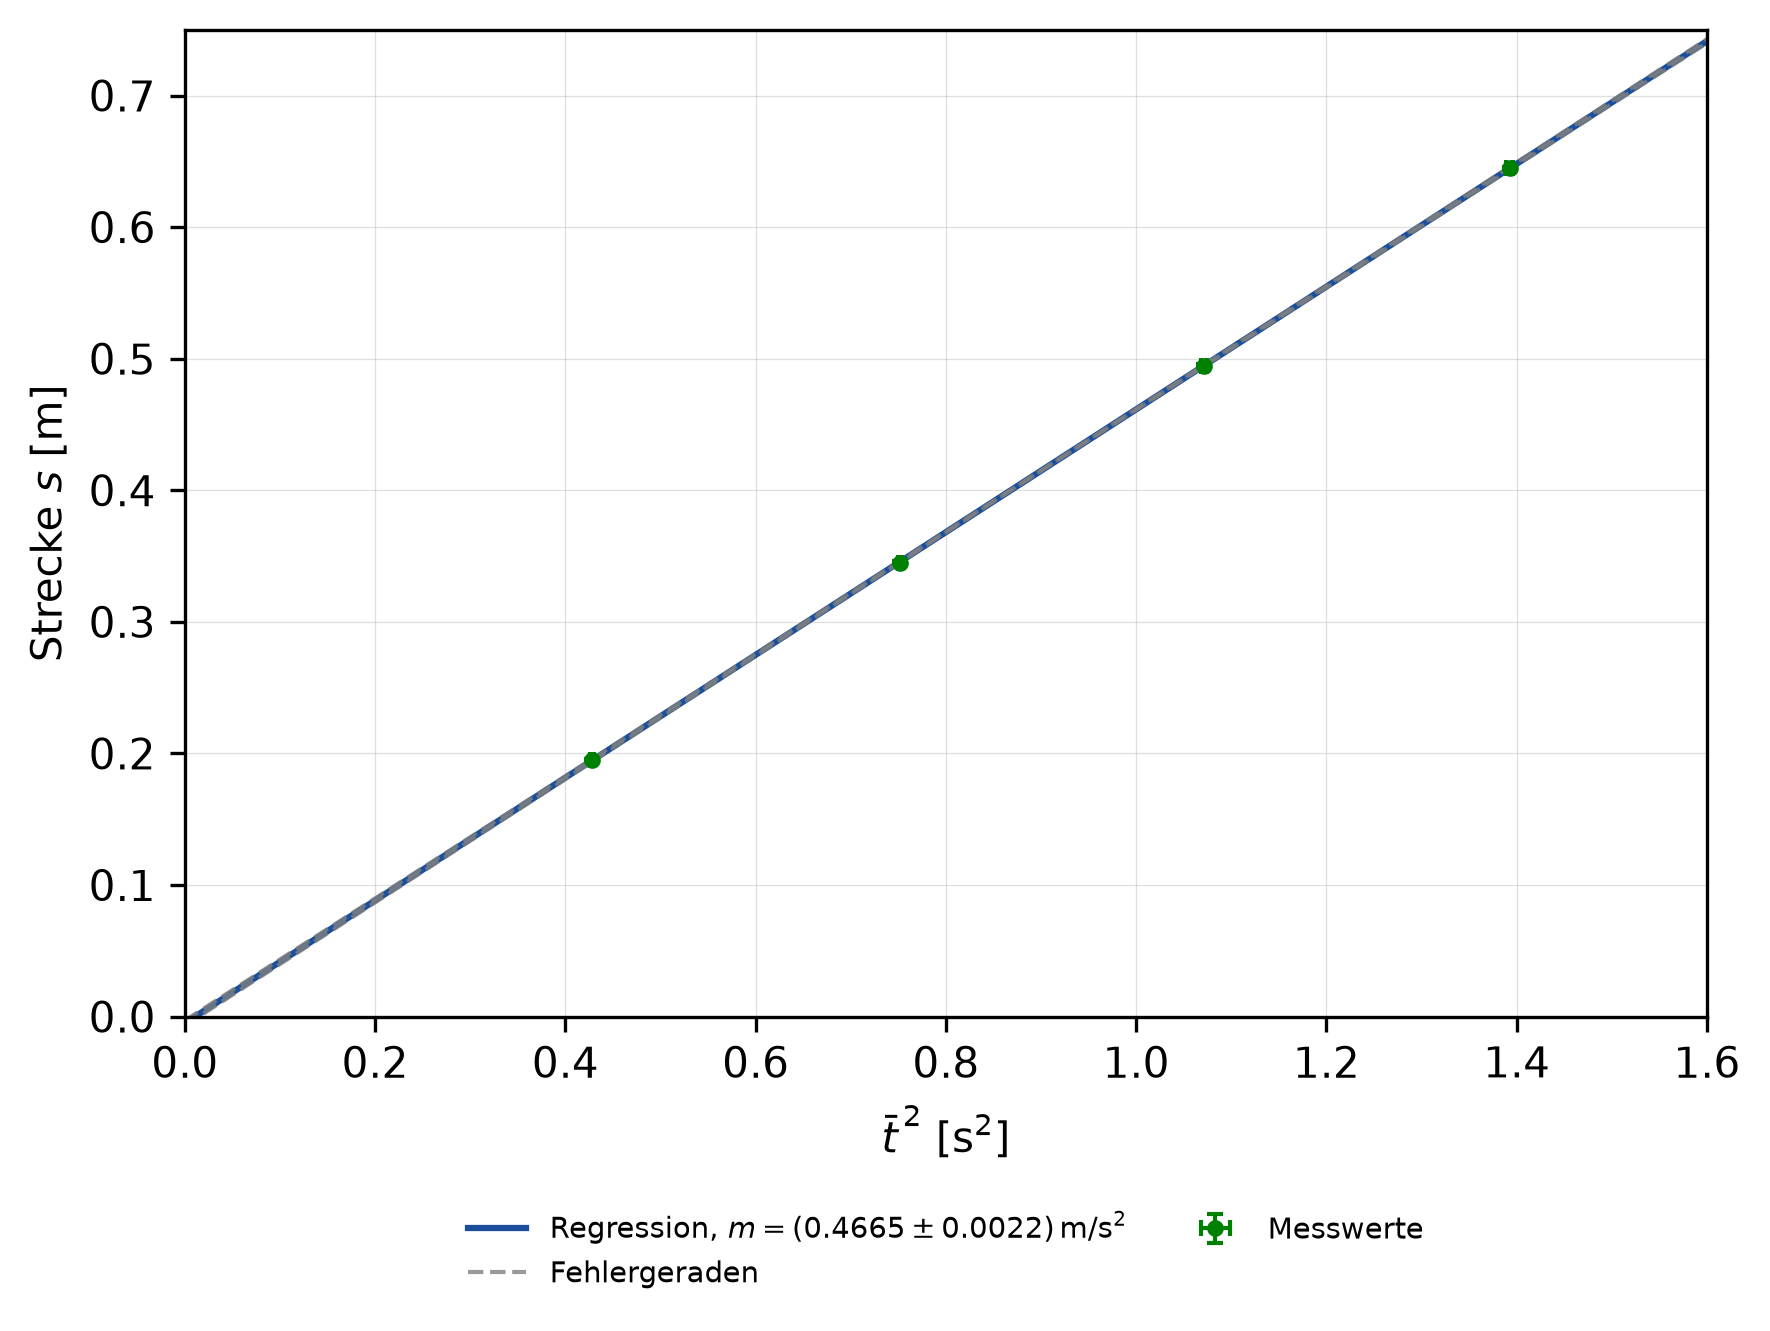
\includegraphics[width=0.75\textwidth]{export/diagramme/s_t2.png}
	\caption{Strecke $s$ über $\bar t^{\,2}$ mit gewichteter Regression und Fehlergeraden}
	\label{fig:s-t2}
\end{figure}

Die Regression liefert $m = \erg{fit_V_m}$ und $b = \erg{fit_V_b}$. Mit
\begin{align}
  a_\mathrm{V} &= 2 m \label{eq:a_V} \\
  \Delta a_\mathrm{V} &= \left|\frac{\partial a_\mathrm{V}}{\partial m}\right| \Delta m \nonumber \\
  &= 2\,\Delta m \label{eq:da_V}
\end{align}

folgt
\begin{equation*}
	\boxed{a_\mathrm{V} = \erg{a_V}}
\end{equation*}
Dieser Wert weicht um \ergsig{a_V_th}\,$\sigma$ von $a_\mathrm{th}$ ab.
% ======================================================================


\section{Diskussion}
\label{sec:diskussion}


\section{Anhang}
\label{sec:anhang}


\end{document}
